\documentclass[12pt]{article} 
\usepackage{longtable}
\usepackage{makecell}
\usepackage{float}
\usepackage{graphicx}
\usepackage{bm}
\usepackage{placeins}
\usepackage{booktabs}
\usepackage{gensymb}
\usepackage{amssymb}
\usepackage{indentfirst}
\usepackage{threeparttable} 
\usepackage{multirow}
\usepackage{subfigure} % 导言区引入
\usepackage{tabularx}
\usepackage{aligned-overset}
\usepackage[slantfont,boldfont]{xeCJK}
\usepackage{fontspec}
\renewcommand{\arraystretch}{1.5}
% \usepackage[paperwidth=21cm,paperheight=29.7cm]{geometry}
\usepackage[a4paper,margin=2cm]{geometry}
\setCJKmainfont{SimSun}
\setmainfont{SimSun}
\setsansfont{SimSun}
% 设置正文字体为四号（12pt）
% \renewcommand{\CJKmainfont}{SimSun}
\renewcommand{\CJKfamilydefault}{\CJKrmdefault}
\renewcommand{\normalsize}{\fontsize{12pt}{18pt}\selectfont}
\normalsize

\title{棱镜色散实验报告}
\author{2411545 邱凯锐}
\date{2025.11.7}

\begin{document}
\maketitle

\section{实验目的}
1.了解分光仪的结构原理和调节方法

2.测量棱镜的色散

3.了解最小二乘法在曲线拟合中的应用

\section{实验仪器}
分光仪、玻璃棱镜、平面反射镜、低压汞灯。

\section{实验内容}

\subsection{调节分光仪}
利用半透半反镜和各半调节法，将分光仪恢复至可测量的状态。

\subsection{调节待测棱镜}
对放置在载物台上的棱镜应满足下列两个条件： 

（1）平行光束在棱镜的主截面内传播。 

（2）棱镜的主截面必须与刻度盘平行，即棱镜的主截面垂直与仪器
的转轴。这是准确测量主截面内的角度所必须的。 

要达到上述两个要求，首先必须完成对分光仪状态的恢复，这时望
远镜和平行光管的光轴都垂直于仪器转轴，那么当棱镜的两个光学表面
与望远镜垂直时，棱镜主截面也就与仪器的转轴垂直了。因此，仍然用
望远镜作为标准来调节棱镜。注意在用望远镜调节棱镜的过程中，不能
改变已调节好的望远镜状态，否则所建立的标准就被破坏了。将棱镜放
置在载物台上时，应按照 Figure 1 中的方式放置。棱镜的一个光学表面 AB
与载物台的倾斜调节螺丝 $V_1$、$V_3$ 的连线垂直。首先将AB面对准望远镜，
调节 $V_1$（或$V_3$），使 AB 面反射的叉丝象与叉丝重合。然后使载物台与
游标盘锁定，使它们同时绕仪器的转轴转动，转动游标盘让AC面对准
望远镜，调节 $V_2$ 改变AC面的俯仰，使 AC面反射的叉丝象与叉丝重合。
反复对AB面AC面校验几次，直至两个面的反射叉丝象都很好地与叉
丝重合为止。这时两个光学表面均与望远镜的光轴垂直，棱镜达到了测
量所需的要求。

\begin{figure}[H]
    \centering
    
\includegraphics[width=0.5\textwidth]{fig1.png}
    \caption{棱镜的放置方法}
\end{figure}


\subsection{测量棱镜的顶角}

玻璃棱镜的顶角一般为 $60^\circ$，但是在加工时，并不能保证是严格的
$60^\circ$。为了对棱镜进行精确地测量，必须测量棱镜的顶角。如 Figure 2 所示，
测量棱镜顶角的方法有两种。测量是在分光仪和棱镜均已调整好的前题
下进行的。
Figure 2(a) 的方法是利用望远镜进行的，保持望远镜的位置不动，点亮
望远镜的小灯，将载物台与游标盘固定在一起，转动游标盘先使AB面
反射的叉丝象与叉丝重合，然后再转动游标盘使AC面反射的叉丝象与
叉丝重合，这时游标盘转过的角度就是 $\varphi$ ，则顶角为
\begin{equation}
    a=180^\circ-\varphi
\end{equation} 

\begin{figure}[H]
    \centering
    
\includegraphics[width=0.6\textwidth]{fig2.png}
    \caption{测量棱镜的顶角}
\end{figure}

Figure 2(b) 的方法是同时利用平行光管和望远镜进行的。平行光管出射
的平行光同时时照射在AB和AC面上，用望远镜测定两个面上反射光
的传播方向之间的夹角。这个夹角就是 $2a$。 

\subsection{利用最小偏向角测量折射率}
测量棱镜对汞灯在可见光波段的几个不同波长谱线的最小偏向角。
实验方法如 Figure 3 所示。将棱镜的顶角放置在载物台的中心，汞灯的光
经平行光管成为平行
光，各种不同波长的光
以相同的入射角照射到
棱镜上。测量最小偏向
角时，将载物台与游标
盘锁定在一起，使得载
物台与游标盘同时转
动。先用眼睛寻找折射
后的狭缝象，找到后再将望远镜移动眼睛所在的位置。此时就能看到汞
灯的光谱谱线。然后通过转动游标盘朝任意稍微转动棱镜，观察谱线移
动的方向，判断偏向角是增大还是减小。然后还是通过转动游标盘转动
棱镜，使谱线向偏向角减小的方向移动，这时应保持所观测的谱线始终
在望远镜的视场中。当棱镜被转到某一位置时，谱线中的一条会达到一
个转折位置，此时无论棱镜向那个方向转，这条谱线的偏向角均往偏向
角增大方向移动。这个转折点就是棱镜对于该谱线处于最小偏向角的位
置。这时锁定游标盘和载物台，使它们不能转动。再利用载物台的微调
螺丝稍微转动载物台，确认棱镜确实处在最小偏向角位置。将望远镜与
刻度盘锁定在一起，使它们同时转动。转动望远镜让叉丝对准谱线。从
两个游标上读出望远镜所处的位置，即最小偏向位置。
再转动望远镜让它的叉丝对准平行光管的狭缝，
从游标上读出入射光位置。同一游标上两个位置之差就是棱镜对该谱线
的最小偏向角。但存在偏心差，两个游标所得到的结果的算术平均值才
是实际的最小偏向角。

\begin{figure}[H]
    \centering
    
\includegraphics[width=0.6\textwidth]{fig3.png}
    \caption{偏向角的测量方法}
\end{figure}

分别测量所能看到的各个谱线的最小偏向角。汞灯的谱线波长和相
对强度列于 Table 1 中。

\begin{table}[h]
\centering
\caption{汞灯谱线的波长}
\begin{tabular}{|c|c|c|c|c|c|c|c|}
\hline
波长 (nm) & 579.1 & 577.0 & 546.1 & 491.6 & 435.8 & 407.8 & 404.7 \\ \hline
颜色 & 黄 & 黄 & 绿 & 深绿 & 蓝 & 紫 & 紫 \\ \hline
相对强度 & 强 & 强 & 强 & 弱 & 强 & 弱 & 强 \\ \hline
\end{tabular}
\end{table}

\subsection{求棱镜材料的折射率与波长的关系及色散率}
在某一波长的光以最小偏向角的
方式通过棱镜，棱镜材料对该波长的折射率与棱镜顶角 $a$ 和最小偏向角 $\delta$
的之间的关系为：
\begin{equation}
    n=\frac{\sin[(a+\delta)/2]}{\sin(a/2)}
\end{equation}

因此，由前面测定的 $a$ 和 $\delta$ 就可以得到 $n$，对于光学玻璃，其折射率
与波长的关系可以由科西公式描述，
\begin{equation}
    n=A+\frac{B}{\lambda^2}+\frac{C}{\lambda^4}
\end{equation}
式中，波长的单位为nm，A、B、C是光学玻璃特性所决定的。我们可以利用最小二乘法确定这三个系数。

假定对应测量点的波长，其折射率的真值为 $\hat n_1$,$\hat n_2$,$\cdots$,$\hat n_m$，则有
\begin{equation}
    \hat n_i=A+B\lambda_i^{-2}+C\lambda_i^{-4},\quad i=1,2,\cdots,m
\end{equation}
而测量数据 $n_1$,$n_2$,$\cdots$,$n_m$的残差应为
\begin{equation}
    n_i-\hat n_i=e_i,\quad i=1,2,\cdots,m
\end{equation}
即
\begin{equation}
    n_i-(A+B\lambda_i^{-2}+C\lambda_i^{-4})=e_i,\quad i=1,2,\cdots,m 
\end{equation}
按照最小二乘原理
\begin{equation}
    Q=\sum_ie_i^2=\min
\end{equation}
对各个参数做偏导，有
\begin{equation}
    \begin{aligned}
        \frac{\partial Q}{\partial A}&= mA+\sum_i \lambda_i^{-2}B+\sum_i \lambda_i^{-4}C-\sum_i n_i &=0\\
        \frac{\partial Q}{\partial B}&= \sum_i \lambda_i^{-2}A +\sum_i \lambda_i^{-4}B+\sum_i \lambda_i^{-6}C-\sum_i \lambda_i^{-2} n_i &=0\\
        \frac{\partial Q}{\partial C}&= \sum_i \lambda_i^{-4}A +\sum_i \lambda_i^{-6}B+\sum_i \lambda_i^{-8}C-\sum_i \lambda_i^{-4} n_i &=0
    \end{aligned}
\end{equation}
即
\begin{equation}
    \begin{aligned}
        mA+\sum_i \lambda_i^{-2}B+\sum_i \lambda_i^{-4}C&=\sum_i n_i\\
        \sum_i \lambda_i^{-2}A +\sum_i \lambda_i^{-4}B+\sum_i \lambda_i^{-6}C&=\sum_i \lambda_i^{-2} n_i \\
        \sum_i \lambda_i^{-4}A +\sum_i \lambda_i^{-6}B+\sum_i \lambda_i^{-8}C&=\sum_i \lambda_i^{-4} n_i 
    \end{aligned}
\end{equation}
求解方程，即可确定 $A$,$B$,$C$ 三个系数。

\section{实验数据}
\subsection{棱镜的顶角}
\begin{table}[H]
\centering
\caption{顶角测量数据与平均值}
\begin{tabular}{ccccc}
\hline
次数 & 游标编号 & 位置1 & 位置2 & 顶角 \\ \hline
\multirow{2}{*}{1} & 1 & 35°49′ & 155°53′ & \multirow{2}{*}{60°2′} \\ \cline{2-4}
  & 2 & 215°53′ & 335°53′ &  \\ \hline
\multirow{2}{*}{2} & 1 & 46°22′ & 166°26′ & \multirow{2}{*}{60°2′} \\ \cline{2-4}
  & 2 & 226°25′ & 346°29′ &  \\ \hline
\multirow{2}{*}{2} & 1 & 57°17′ & 177°17′ & \multirow{2}{*}{60°0′} \\ \cline{2-4}
  & 2 & 237°18′ & 357°19′ &  \\ \hline
\end{tabular}
\end{table}


得到 $\overline a=60^\circ1'$
\subsection{最小偏向角}
\begin{table}[H]
\centering
\caption{不同波长下的最小偏向角测量结果}
\renewcommand{\arraystretch}{1.2}
\setlength{\tabcolsep}{6pt}
\begin{tabular}{>{\centering\arraybackslash}m{1.8cm}
                >{\centering\arraybackslash}m{1.5cm}
                >{\centering\arraybackslash}m{2.5cm}
                >{\centering\arraybackslash}m{2.5cm}
                >{\centering\arraybackslash}m{2cm}
                >{\centering\arraybackslash}m{2.5cm}}
\toprule
波长 (nm) & 游标编号 & 最小偏向角位置 & 入射光角度 & 最小偏向角 & 消除偏心差的最小偏向角 \\
\midrule
\multirow{2}{*}{579.1} & 1 & $20^\circ0'$ & $326^\circ18'$ & $53^\circ42'$ & \multirow{2}{*}{$53^\circ40'$} \\\cline{2-5}
                       & 2 & $200^\circ4'$ & $146^\circ22'$ & $53^\circ38'$ &  \\[3pt]
\midrule
\multirow{2}{*}{577.0} & 1 & $20^\circ4'$ & $326^\circ16'$ & $53^\circ48'$ & \multirow{2}{*}{$53^\circ44'$} \\\cline{2-5}
                       & 2 & $200^\circ20'$ & $146^\circ40'$ & $53^\circ40'$ &  \\[3pt]
\midrule
\multirow{2}{*}{546.1} & 1 & $20^\circ28'$ & $326^\circ28'$ & $55^\circ0'$ & \multirow{2}{*}{$54^\circ30'$} \\\cline{2-5}
                       & 2 & $200^\circ29'$ & $146^\circ29'$ & $54^\circ0'$ &  \\[3pt]
\midrule
\multirow{2}{*}{435.8} & 1 & $20^\circ58'$ & $326^\circ0'$ & $54^\circ58'$ & \multirow{2}{*}{$54^\circ59'$} \\\cline{2-5}
                       & 2 & $201^\circ0'$ & $146^\circ0'$ & $55^\circ0'$ &  \\[3pt]
\midrule
\multirow{2}{*}{404.7} & 1 & $21^\circ9'$ & $324^\circ45'$ & $56^\circ24'$ & \multirow{2}{*}{$56^\circ24.5'$} \\\cline{2-5}
                       & 2 & $201^\circ15'$ & $144^\circ50'$ & $56^\circ25'$ &  \\[3pt]
\bottomrule
\end{tabular}
\end{table}

\subsection{各波长对应的折射率}

\begin{table}[H]
    \centering
    \caption{不同波长下的折射率}
    \renewcommand{\arraystretch}{1.2}
    \setlength{\tabcolsep}{8pt}
    \begin{tabular}{cccccc}
        \toprule
        波长 $\lambda$ (nm) & 579.1 & 577.0 & 546.1 & 435.8 & 404.7 \\ 
        \midrule
        折射率 $n$ & 1.6739 & 1.6745 & 1.6818 & 1.6864 & 1.6996 \\ 
        \bottomrule
    \end{tabular}
\end{table}

\subsection{确定棱镜玻璃所用材料的柯西公式}

利用所得到的折射率测量结果代入公式（9）确定科西公式中的三
个系数。在坐标纸上以波长作横轴，折射率作纵轴，标出实验测量数据，
并利用实验结果确定的系数，代入科西公式画出 $n～\lambda$ 的曲线。观察数据
点与实验曲线的分布关系，试比较作图法与最小二乘法的区别。

\begin{figure}[H]
    \centering
    
\includegraphics[width=0.8\textwidth]{Figure_1.png}
\end{figure}

计算得到 $A=1.6864$ , $B=-8.6672\times 10^{3}$ , $C=1.7389\times 10^{9}$ 。

均方根误差为
\begin{equation}
    \text{RMSE}=2.2\times 10^{-4}
\end{equation}
决定系数
\begin{equation}
    R^2=0.99998
\end{equation}


\section{思考题}

试用实验中棱镜所用的光学玻璃，设计一个实验装置。要求这个实
验装置能够使钠黄光的两个波长（钠黄光的波长为 589.0nm 和
589.6nm）在成象物镜的焦平面上分开1mm。画出实验装置光路图，并注明各元件的参数，给出计算过程。 

两条黄光的折射率分别为
\begin{equation}
    \begin{aligned}
        n_1&=A+\frac{B}{\lambda_1^2}+\frac{C}{\lambda_1^4}=1.675856257\\
        n_2&=A+\frac{B}{\lambda_2^2}+\frac{C}{\lambda_2^4}=1.675848356
    \end{aligned}
\end{equation}
最小偏向角分别为
\begin{equation}
    \begin{aligned}
        \delta_1&=2\arcsin\left(n_1\sin\frac{a}{2} \right)-a=53.87161944^\circ\\
        \delta_2&=2\arcsin\left(n_2\sin\frac{a}{2} \right)-a=53.8707893^\circ
    \end{aligned}
\end{equation}
\begin{equation}
    \Delta\delta=0.00083014^\circ
\end{equation}

实验设计如下：

（1）先用棱镜将两条黄光分离出一个偏角 $\Delta\delta$

（2）使用焦距为 200mm 的透镜，放置于棱镜一倍焦距处，产生平行光，间隔为 
\begin{equation}
    s_0=f\Delta\delta=0.5288\ \mathrm{mm}
\end{equation}

(3)再使用一个放大率为 2 的透镜，即可得到 
\begin{equation}
    s=2s_0=1.0576\ \mathrm{mm}\approx 1\ \mathrm{mm}
\end{equation}

\begin{figure}[H]
    \centering
    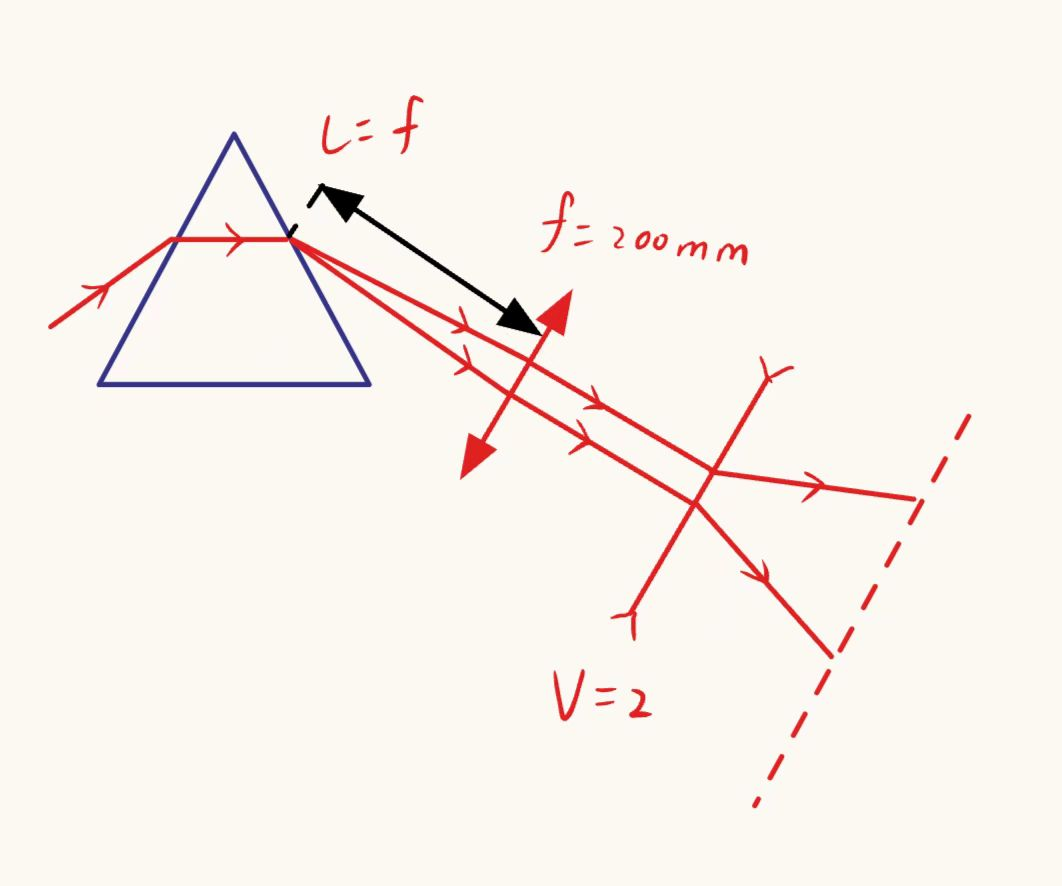
\includegraphics[width=0.6\textwidth]{fff.jpg}
\end{figure}
\end{document}